\documentclass[aspectratio=169,11pt]{beamer}

\usetheme{Madrid}
\usecolortheme{default}
\setbeamertemplate{navigation symbols}{}

\usepackage{amsmath,amssymb,mathtools}
\usepackage{booktabs}
\usepackage{graphicx}
\usepackage{subcaption}
\usepackage{hyperref}
\usepackage{tikz}

\graphicspath{{presentation/img/}{img/}{../report/generated/}{../experiments/demand_understanding/}}

\newcommand{\R}{\mathbb{R}}
\newcommand{\E}{\mathbb{E}}
\newcommand{\cU}{\mathcal{U}}
\DeclareMathOperator*{\argmin}{arg\,min}

\title[Robust Station Selection]{Robust Station Selection for Microtransit Under Demand Uncertainty}
\author[Gabriel Yong]{Gabriel Yong}
\date{}

\begin{document}

\begin{frame}
	\titlepage
\end{frame}

\begin{frame}{What Is Microtransit?}
	\centering
	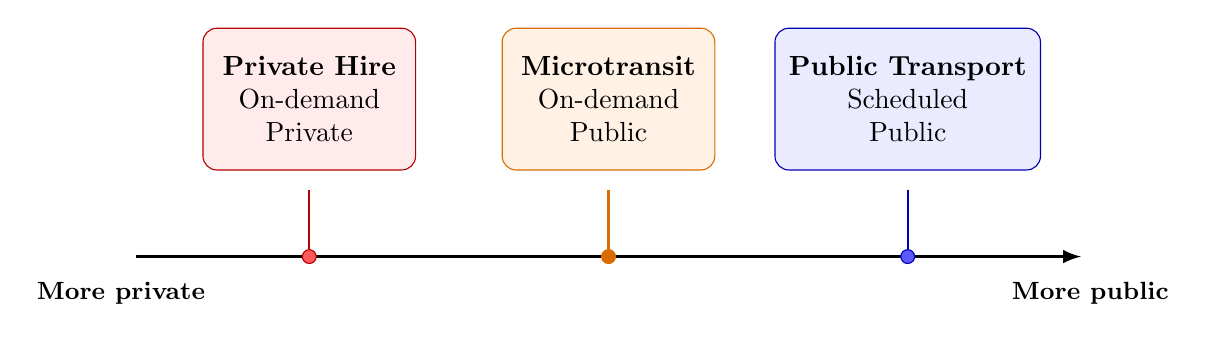
\begin{tikzpicture}[
			x=1cm,
			y=1cm,
			labelbox/.style={draw, rounded corners=5pt, align=center, minimum width=2.7cm, minimum height=1.8cm, inner sep=5pt},
			scale label/.style={font=\small\bfseries}
		]
		\draw[very thick, -latex] (0,0) -- (12,0);
		\node[scale label, anchor=north east] at (1.0,-0.2) {More private};
		\node[scale label, anchor=north west] at (11.0,-0.2) {More public};

		\filldraw[fill=red!65, draw=red!70!black] (2.2,0) circle (2.5pt);
		\node[labelbox, fill=red!8, draw=red!70!black] at (2.2,2.0) {
			\textbf{Private Hire}\\
			On-demand\\
			Private
		};
		\draw[red!70!black, thick] (2.2,0.1) -- (2.2,0.85);

		\filldraw[fill=orange!85!black, draw=orange!85!black] (6,0) circle (2.5pt);
		\node[labelbox, fill=orange!10, draw=orange!85!black] at (6,2.0) {
			\textbf{Microtransit}\\
			On-demand\\
			Public
		};
		\draw[orange!85!black, thick] (6,0.1) -- (6,0.85);

		\filldraw[fill=blue!65, draw=blue!70!black] (9.8,0) circle (2.5pt);
		\node[labelbox, fill=blue!8, draw=blue!70!black] at (9.8,2.0) {
			\textbf{Public Transport}\\
			Scheduled\\
			Public
		};
		\draw[blue!70!black, thick] (9.8,0.1) -- (9.8,0.85);
	\end{tikzpicture}
\end{frame}

\begin{frame}{Problem Setting}
	\begin{itemize}
		\item For Microtransit, it is important to decide where to set a `Virtual Bus Stop'
		\item Virtual bus stop (VBS) selection determines service coverage, and pooling quality in microtransit.
		\item A station plan that is good for nominal demand could be fragile when demand shifts across OD pairs or time periods.
	\end{itemize}
\end{frame}

\begin{frame}{Goal}
	\begin{itemize}
		\item Build a two-stage robust optimization model for station selection under uncertain OD demand.
		\item Protect against plausible demand deviations
		\item Compare nominal and robust plans on out-of-sample service quality.
	\end{itemize}
\end{frame}

\begin{frame}{Two-Stage Model}
	\begin{columns}
		\begin{column}{0.5\textwidth}
			Decision Variables
			\begin{itemize}
				\item First Stage Decision:
				      \begin{itemize}
					      \item Which candidate stations to build: $y_j \in \{0,1\}$
				      \end{itemize}
				\item Second Stage Decisions:
				      \begin{itemize}
					      \item Which candidate stations to activate in scenario $s$:  $z_{js} \in \{0,1\}$
					      \item And which station pair $j, k$ to assign an order coming from $o, d$: $x_{odjks} \in \{0,1\}$
				      \end{itemize}
			\end{itemize}
		\end{column}

		\begin{column}{0.5\textwidth}
			Other coefficients and notations
			\begin{itemize}
				\item Objective is to minimize $a_{odjks} = d^{\mathrm{orig}}_{oj} + d^{\mathrm{dest}}_{dk} + \lambda c_{jk}$
				      \begin{itemize}
					      \item Walking Cost $d_{oj}$, $d_{dk}$
					      \item Routing cost $c_{jk}$
				      \end{itemize}
				\item Number of orders from $o$ to $d$ in scenario $s$: $q_{ods}$
				\item $x_{odjks}$ assignments are restricted to a walking distance limit
				      \begin{itemize}
					      \item $ A_{od} = \{(j,k): j \in \Delta(o),\ k \in \Delta(d)\}$ where $\Delta(o)$ represents the set of stations walkable from $o$
				      \end{itemize}
			\end{itemize}

		\end{column}
	\end{columns}
\end{frame}

\begin{frame}{Nominal Objective and Constraints}
	\small
	\textbf{Nominal objective}
	\[
		\min_{x,y,z}
		\sum_{s \in S}\sum_{(o,d)\in\Omega}\sum_{(j,k)\in A_{od}}
		q_{ods}\, a_{odjks}\, x_{odjks}
	\]

	\textbf{Constraints}
	\begin{align*}
		 & \sum_{(j,k)\in A_{od}} x_{odjks}  = 1                                   &  & \forall (o,d), s                 \\
		 & x_{odjks}                         \le z_{js},\quad x_{odjks} \le z_{ks} &  & \forall (o,d),(j,k)\in A_{od}, s \\
		 & z_{js}                            \le y_j                               &  & \forall j, s                     \\
		 & \sum_j y_j                        = l,\quad \sum_j z_{js} = k           &  & \forall s
	\end{align*}

	\begin{itemize}
		\item Every OD pair must be assigned to one feasible station pair.
		\item Assignments can only use active stations, and active stations must be built.
		\item \(l\): number of built stations, \(k\): number of active stations per scenario.
	\end{itemize}
\end{frame}

\begin{frame}{Demand Uncertainty Set}
	\small
	For each scenario \(s\), demand lies in
	\[
		\cU_s =
		\left\{
		q_s :
		\underline{q}_{ods} \le q_{ods} \le \overline{q}_{ods}\ \forall (o,d),\;
		\sum_{(o,d)\in\Omega} q_{ods} \le \overline{Q}_s
		\right\}
	\]

	\begin{itemize}
		\item Each OD demand is bounded between \(\underline{q}_{ods}\) and \(\overline{q}_{ods}\).
		\item Total scenario demand is capped by \(\overline{Q}_s\).
		\item In principle \(q\) is integer-valued, but since the bounds are integer, we relax \(\cU_s\) to be continuous without changing the worst-case value.
	\end{itemize}
\end{frame}

\begin{frame}{Robust Counterpart}
	\textbf{Robust objective}
	\[
		\min_{y,z} \sum_{s \in S} \max_{q_s \in \cU_s} \Phi_s(z_s,q_s)
	\]
	where
	\[
		\Phi_s(z_s,q_s)
		=
		\min_x
		\sum_{(o,d)\in\Omega}\sum_{(j,k)\in A_{od}}
		q_{ods}\, a_{odjks}\, x_{odjks}
	\]

	Dualizing the inner maximization gives
	\[
		\min_{x,y,z,\alpha,\beta,\gamma,t}
		\sum_s \overline{Q}_s\alpha_s
		+ \sum_s\sum_{(o,d)} \overline{q}_{ods}\beta_{ods}
		- \sum_s\sum_{(o,d)} \underline{q}_{ods}\gamma_{ods}
	\]
	\begin{align*}
		\alpha_s + \beta_{ods} - \gamma_{ods} & \ge \sum_{(j,k)\in A_{od}} a_{odjks}x_{odjks} & \forall (o,d), s
	\end{align*}

\end{frame}

\begin{frame}{Calibration of \(\overline{q}\) and \(\overline{Q}\)}
	\small
	\begin{itemize}
		\item Split demand into four time-of-day scenarios: morning, afternoon, evening, night.
		\item For each period \(s\) and OD pair \((o,d)\), aggregate historical requests into daily OD counts.
		\item Set lower bounds to zero:
		      \[
			      \underline{q}_{ods} = 0
		      \]
		\item Estimate OD upper bounds using empirical quantiles of zero-padded daily OD counts:
		      \[
			      \overline{q}_{ods} = \mathrm{Quantile}_q\bigl(\text{daily OD counts in period } s\bigr)
		      \]
		\item Estimate the scenario cap using the same quantile on total period demand:
		      \[
			      \overline{Q}_s = \mathrm{Quantile}_q\bigl(\text{daily total demand in period } s\bigr)
		      \]
	\end{itemize}
\end{frame}

\begin{frame}{Experiment Instance}
	\centering
	\includegraphics[height=0.74\textheight,keepaspectratio]{zhuzhou_sparse40_station_map.png}

	\vspace{0.4em}
	\small Sparse Zhuzhou network used in the main comparison study
\end{frame}


\begin{frame}{Data and Experimental Design}

	\begin{table}
		\centering
		\small
		\begin{tabular}{ll}
			\toprule
			Item                 & Setting                      \\
			\midrule
			Calibration window   & April 1--3, 2025             \\
			Test window          & May 1--31, 2025              \\
			Candidate stations   & \(l = 30\)                   \\
			Active stations      & \(k \in \{10,15,20\}\)       \\
			Walking limit        & 300 seconds                  \\
			Routing weight       & \(\lambda = 10\)             \\
			Robust calibration   & \(q \in \{0.90,0.95,0.99\}\) \\
			In-sample orders     & 2,560                        \\
			Out-of-sample orders & 30,100                       \\
			\bottomrule
		\end{tabular}
	\end{table}
\end{frame}


% \begin{frame}{Dataset Variants}
% 	\begin{table}
% 		\centering
% 		\small
% 		\begin{tabular}{lrrr}
% 			\toprule
% 			Metric                & Full Zhuzhou & Sampled & Sparse \\
% 			\midrule
% 			Stations              & 84           & 40      & 40     \\
% 			Directed segments     & 6,972        & 1,560   & 1,560  \\
% 			April orders          & 2,741        & 2,560   & 2,560  \\
% 			April ODs with orders & 473          & 389     & 130    \\
% 			May orders            & 31,546       & 30,100  & 30,100 \\
% 			May ODs with orders   & 1,412        & 949     & 131    \\
% 			\bottomrule
% 		\end{tabular}
% 	\end{table}
% 
% 	\begin{itemize}
% 		\item The sparse 40-station instance is the main comparison setting.
% 		\item It preserves most order volume while substantially shrinking observed OD support.
% 	\end{itemize}
% \end{frame}


\begin{frame}{Sampled-Network Results}
	\begin{table}
		\centering
		\tiny
		\resizebox{\textwidth}{!}{%
			\begin{tabular}{lllccccc}
				\toprule
				\(k\) & \(q\) & Model   & April mean cost  & May mean cost    & April std.       & May std.         & Uncovered  \\
				\midrule
				10    & --    & Nominal & \textbf{4266.09} & \textbf{4333.42} & 1129.72          & 1116.39          & \textbf{0} \\
				10    & 0.90  & Robust  & 4287.81          & 4359.76          & 1111.08          & 1102.67          & \textbf{0} \\
				10    & 0.95  & Robust  & 4302.24          & 4392.66          & \textbf{1108.89} & \textbf{1090.17} & \textbf{0} \\
				10    & 0.99  & Robust  & 4293.94          & 4369.71          & 1109.24          & 1098.48          & \textbf{0} \\
				\midrule
				15    & --    & Nominal & \textbf{3977.09} & \textbf{4049.94} & 1145.30          & 1119.97          & \textbf{0} \\
				15    & 0.90  & Robust  & 4018.31          & 4071.27          & 1106.48          & 1088.71          & \textbf{0} \\
				15    & 0.95  & Robust  & 4023.38          & 4080.47          & 1105.51          & 1085.45          & \textbf{0} \\
				15    & 0.99  & Robust  & 4030.38          & 4067.03          & \textbf{1096.25} & \textbf{1066.90} & \textbf{0} \\
				\midrule
				20    & --    & Nominal & \textbf{3924.95} & 3984.77          & 1168.67          & 1142.49          & \textbf{0} \\
				20    & 0.90  & Robust  & 3967.29          & 4003.44          & \textbf{1116.51} & \textbf{1082.44} & \textbf{0} \\
				20    & 0.95  & Robust  & 3948.96          & \textbf{3978.06} & 1118.75          & 1090.00          & \textbf{0} \\
				20    & 0.99  & Robust  & 3958.28          & 4005.45          & 1118.56          & 1091.22          & \textbf{0} \\
				\bottomrule
			\end{tabular}%
		}
	\end{table}

\end{frame}

\begin{frame}{Lack of Data Coverage}
	\begin{itemize}
		\item In demand estimation, it is typical that the data might not be as good and so coverage might be lacking when we solve the Nominal model
		\item In an attempt to give the robust model an edge, the request data was filtered down to the top 10\% of origin-destination pairs
		\item This was to compare the coverage scheme of the Robust model
	\end{itemize}
\end{frame}

\begin{frame}{Main Sparse-Network Results}
	\begin{table}
		\centering
		\tiny
		\resizebox{\textwidth}{!}{%
			\begin{tabular}{lllccccc}
				\toprule
				\(k\) & \(q\) & Model   & April mean cost  & May mean cost    & April std.      & May std.         & Uncovered  \\
				\midrule
				10    & --    & Nominal & \textbf{4446.97} & \textbf{4305.57} & 851.46          & 1092.41          & 227        \\
				10    & 0.90  & Robust  & 4505.20          & 4363.35          & 845.97          & 1100.00          & \textbf{0} \\
				10    & 0.95  & Robust  & 4521.04          & 4392.62          & \textbf{836.33} & 1094.39          & \textbf{0} \\
				10    & 0.99  & Robust  & 4507.51          & 4368.66          & 840.04          & \textbf{1089.52} & \textbf{0} \\
				\midrule
				15    & --    & Nominal & \textbf{4182.48} & \textbf{4031.55} & 881.21          & 1082.65          & 14         \\
				15    & 0.90  & Robust  & 4234.00          & 4080.66          & 853.99          & 1059.06          & \textbf{0} \\
				15    & 0.95  & Robust  & 4235.88          & 4089.67          & \textbf{848.30} & \textbf{1058.01} & \textbf{0} \\
				15    & 0.99  & Robust  & 4236.58          & 4073.98          & 855.82          & 1067.54          & \textbf{0} \\
				\midrule
				20    & --    & Nominal & \textbf{4136.13} & \textbf{3972.53} & 901.73          & 1094.37          & \textbf{0} \\
				20    & 0.90  & Robust  & 4149.90          & 3985.01          & 886.97          & 1082.80          & \textbf{0} \\
				20    & 0.95  & Robust  & 4155.78          & 3998.38          & \textbf{883.00} & \textbf{1077.17} & \textbf{0} \\
				20    & 0.99  & Robust  & 4148.22          & 3984.41          & 887.77          & 1079.39          & \textbf{0} \\
				\bottomrule
			\end{tabular}%
		}
	\end{table}
\end{frame}

\begin{frame}{Sparse Results: Cost CDFs at \(k=15\)}
	\centering
	\begin{columns}[c]
		\column{0.48\textwidth}
		\centering
		\includegraphics[width=\textwidth]{cdf_k15_period_1.png}

		\small Morning (06--10h)

		\column{0.48\textwidth}
		\centering
		\includegraphics[width=\textwidth]{cdf_k15_period_2.png}

		\small Afternoon (10--15h)
	\end{columns}
\end{frame}

\begin{frame}{Sparse Results: Activations at \(k=10\)}
	\centering
	\begin{columns}[c]
		\column{0.48\textwidth}
		\centering
		\includegraphics[width=0.75\textwidth]{activation_nominal_period_1_k10.png}

		\small Nominal, morning

		\column{0.48\textwidth}
		\centering
		\includegraphics[width=0.75\textwidth]{activation_robust_q095_period_1_k10.png}

		\small Robust (\(q=0.95\)), morning
	\end{columns}
\end{frame}

% \begin{frame}{Interpretation of Results}
% 	\begin{itemize}
% 		\item Nominal has the lowest April mean cost for every \(k\), so it fits the sparse training data best.
% 		\item At \(k=10\) and \(k=15\), nominal leaves uncovered May orders; robust models achieve full coverage.
% 		\item Robust variants trade higher April mean cost for better coverage and slightly lower May variability.
% 		\item By \(k=20\), all models cover every order and mean costs are very close.
% 	\end{itemize}
% \end{frame}


\begin{frame}{Conclusion}
	\begin{itemize}
		\item A budgeted uncertainty set gives a practical way to model uncertain OD demand without extreme conservatism.
		\item Robustness guarantees coverage but alternative ways such as enforcing through constraints could be more efficient
	\end{itemize}
	Future Exploration
	\begin{itemize}
		\item Recourse function is overly simplistic in this model and does not reflect true microtransit operations
		\item Understanding which specific scenarios make having a Robust solution necessary, such as in significantly lower demand areas
	\end{itemize}
\end{frame}

\end{document}
